\documentclass[twocolumn, 9pt, a4j, dvipdfmx]{jsarticle}
%
\usepackage[top=20truemm,bottom=20truemm,left=16truemm,right=16truemm]{geometry}

%
\usepackage{url}
\usepackage{amsmath,amssymb}
\usepackage{type1cm}
\usepackage{color}
\usepackage{bm}
\usepackage{graphicx}
\usepackage{subfigure}
\usepackage{verbatim}
\usepackage{wrapfig}
\usepackage{ascmac}
\usepackage{makeidx}
\usepackage{enumerate}
\usepackage{algorithm}
\usepackage{algpseudocode}
\usepackage{multicol}
%
\usepackage{caption}
\captionsetup[figure]{format=plain, labelformat=simple, labelsep=period, font=bf}
\captionsetup[table]{format=plain, labelformat=simple, labelsep=period, font=bf}

%
\newcommand{\argmax}{\mathop{\rm arg~max}\limits}
\newcommand{\argmin}{\mathop{\rm arg~min}\limits}
\newcommand{\median}{\mathop{\rm \text{median}}\limits}
% \newcommand{\red}[1]{{#1}}
\newcommand{\red}[1]{\textcolor{red}{#1}}
% \newcommand{\diff}{\mathrm{d}}  %微分記号
% \newcommand{\divergence}{\mathrm{div}\,}  %ダイバージェンス
% \newcommand{\grad}{\mathrm{grad}\,}  %グラディエント
% \newcommand{\rot}{\mathrm{rot}\,}  %ローテーション
%

\pagestyle{empty}
\title{
    キーポイントパッチ抽出法を用いた\\
    三次元点群レジストレーションに関する諸検討
}
\author{16T2806E 齊藤 陽平}
\date{\today}

\begin{document}
\maketitle
\section{研究背景}
三次元点群はコンピュータビジョンの一分野であり, 
物体を複数の離散的な点で表現したものである.
近年では三次元点群の取得できる安価なセンサの普及により
モデリングやロボディクス, 測量などの分野で三次元点群の
技術に対する需要が高くなっている. 
特に三次元点群処理は構成する点の数が莫大になり計算コストが高くなるため, 
高能率な手法が求められている.

実空間上の物体をレーザなどで測定し点群化するとき,
物体の影や裏側にはレーザが届かず一回で完全に物体の全面を一つの点群として
構成する計測は不可能である.
そのため完全なモデルを作成するには
複数の位置から取得した点群を一つの点群にまとめる必要がある. 
このように複数の点群の相対関係を決定する問題をレジストレーションという. 
本稿ではレジストレーションにおいて重ねる基準となる点群をターゲット点群
($\mathcal{T}=\{\bm{q_1}, \bm{q_2}\ldots\bm{q_{N_t}}\}$)
ターゲット点群に重なる点群をソース点群
($\mathcal{S}=\{\bm{p_1}, \bm{p_2}\ldots\bm{p_{N_s}}\}$)とする. 
レジストレーションのイメージを図\ref{registration}に示す. 
ここで赤色がターゲット点群であり, 青色がソース点群である. 
同一空間上にそのまま点をプロットすると左のように, 
点分布の向きが揃わないが, レジストレーションを行うことで右のように
2つの点群が一つの形状にまとまる. 
\vspace{-2mm}
\begin{figure}[H]
    \centering
    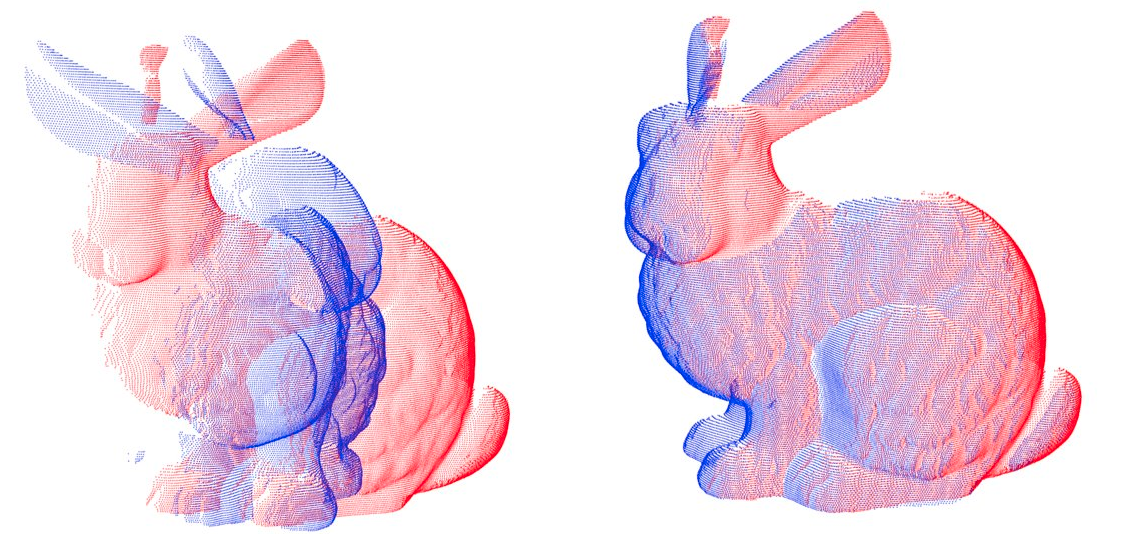
\includegraphics[clip, width=0.8\linewidth]{./img/registration.png}
    \caption{レジストレーションのイメージ\label{registration}}
\end{figure}
\vspace{-5mm}
\section{レジストレーション手法と先行研究}
代表的なレジストレーションの手法にはICP, 特徴点のマッチング, 進化計算(ECR)など
が挙げられる. 
中でもECRでは精度や成功確率が高い一方で
計算時間が長いというデメリットが存在する. 
進化計算レジストレーションでは式(\ref{FS})の評価関数を最小化する事で, 
最適な重なりとなる剛体変換$f$を求める.
ここで, 剛体変換$f$を構成するのに必要な要素は
$(\theta_x, \theta_y, \theta_z ,t_x, t_y, t_z)$の6次元であり, 
進化計算の遺伝子もこの6次元ベクトルである. 
\begin{equation}
    \label{FS}
    FS = \frac{1}{N_s} \sum_{\bm{p}_i \in \mathcal{S}}
        \| f(\bm{p}_i) - \argmin_{\bm{q}_j \in\mathcal{T}}(f(\bm{p}_i) - \bm{q}_j) \|^2
\end{equation}
計算時間が長い理由は評価関数で用いられる最近傍探索の回数が
$個体数 \times 世代数 \times N_s$と非常に多くなってしまうためである. 
そこで植西ら\cite{KPP}はキーポイントパッチ(KPP)抽出法によるECR(KPP-ECR)を提案した.
この手法ではソース点群をキーポイントとその周辺の点に限定することで, 
ECRを100倍程度の高速化に成功した. 
しかし, 
KPP-ECRでは点群同士重なりのない場所にKPPを抽出すると
そのKPPがターゲット点群に引きつけられるため, 
成功可能かどうかがKPPの位置に深く関係する.
しかし, 従来法ではKPPの位置に対しての最適な配置に関する考察は未だなされていない. 
本稿ではこのKPPの位置を自動的に補正する方法について提案と
その評価・考察を記す.
\section{提案法}
本提案法では予めキーポイントパッチを大量に抽出し, 
その中から使用するパッチを適宜選択することで , 
キーポイントパッチの位置を最適化の過程で変化させる.
各世代で評価関数が変動するため, 進化計算手法にはCMA-ES\cite{CMA-ES}を用いる. 
提案法は次のようなステップで実行する. 
\begin{itembox}[l]{提案手法のフロー}
\vspace{-2mm}
\begin{enumerate}[Step1.]
    \item キーポイント周囲の点をパッチ集合$\mathcal{A}$として抽出する
    \item CMA-ESのパラメータを設定する
    \item CMA-ESの平均を用いて, パッチを評価する 
    \item パッチの評価値からパッチ集団を更新する 
    \item パッチ集団の中から評価に使うパッチ$\mathcal{U}$を選択する 
    \item CMA-ESで生成した個体をソース点群を$\mathcal{U}$として評価する
    \item CMA-ESのパラメータを更新する 
    \item 収束条件ならば終了, そうでなければStep3.に戻る
\end{enumerate}
\vspace{-2mm}
\end{itembox}
Step3. パッチの評価では1世代に一度パッチ$\mathcal{A}_i$毎に
式(\ref{FS_PATCH})によって評価値を求める. 
ここで$cl$は$p_i$から一番近いターゲット点群の点の番号である. 
$\bm{p}_{(i,n)}$は点$\bm{p}_i$の法線を示す. 
この評価関数では法線による値と距離による値の積で評価を行っている. 
理想的に重なる点群かどうかは形状の情報のみを利用することが望ましい. 
しかし, 形状だけの情報で評価するとターゲット点群の穴の中のパッチが
稀に残ってしまうので今回は距離情報も加味した.
\begin{align}
    \label{FS_PATCH}
    \small
    FS_{p}(\mathcal{A}_i) = 
    \scriptsize
    \sqrt{1 -  
        \frac
        {\sum_{\bm{p}_i \in \mathcal{A}_i}|\bm{p}_{(i,n)} \cdot \bm{q}_{(cl,n)}|}
        {\text{count}(\mathcal{A}_i)} 
    } 
    \sqrt{
        \frac
        {\sum_{\bm{p_i}\in\mathcal{A}_i}\|\bm{p_i} - \bm{q_{cl}}\|^2}
        {\text{count}(\mathcal{A}_i)}
    }
\normalsize
\end{align}

Step4. パッチ集団の更新では世代$g$でのパッチ集団$\mathcal{A}^g$を
式(\ref{restrict},\ref{remove})で更新していく. 
更新によって重ならないパッチを選択肢から除外する. 
ここで$G$は終了世代数, $\bar{\mathcal{A}^g}, \sigma_{\mathcal{A}^g}$はそれぞれ
世代のパッチ評価値の平均, 分散である. 

\begin{align}
    \label{restrict}
    \mathcal{A}^{g+1}=
    \begin{cases}
        remove(\mathcal{A}^g) & N_u < \text{count}(remove(\mathcal{A}^g))\\
        \mathcal{A}^g & otherwise
    \end{cases}
\end{align}
\vspace{-2em}
\begin{align}
    \label{remove}
    remove(\mathcal{A}^g) = \{
        \mathcal{A}^g_i \in \mathcal{A}^g \mid 
        \bar{\mathcal{A}^g} + k\sigma_{\mathcal{A}^g} < FS_p(\mathcal{A}^g_i)
    \}
\end{align}
\vspace{-2em}
\begin{align}
    \label{trim-rate}
    k_g = \alpha + \beta \frac{G-g}{G+g}
\end{align}

Step5. パッチ選択は評価関数に使用するためのパッチを$N_u$個, 選択肢から選択する. 
評価が良いパッチも悪いパッチも選ぶために, 式(\ref{select},\ref{select-idx})
を利用して評価値全体でまんべんなく評価を選択する. 
ここで$\mathcal{A}_i^{(g+1) '}$は
評価値でソートされたパッチ集団$\mathcal{A}_i^{(g+1)}$であり, 
$L_g = \lfloor \frac{\text{count}(\mathcal{A}^{g+1})}{N_u} \rfloor$である. 
このように選択する事で, 一部のパッチのみで収束してしまうことを防ぐ. 
\begin{align}
    \label{select}
    \mathcal{U}^{g+1} = \bigcup_{i \in I^g} \mathcal{A}^{(g+1) '}_i 
\end{align}
\vspace{-2em}
\begin{align}
    \label{select-idx}
    I^g = \{L_g j + rand (0, L_g) | j \in \mathbb{Z} \cap [1, N_u]\}
\end{align}
\vspace{-2em}
\section{実験と結果}
本手法と従来のKPP-ECRで実際にレジストレーションを行った. 
点群にStanfordレポジトリ\cite{stanford}を使用し, 
実装にはPoint Cloud Library\cite{PCL}を使用した. 
実験では時間短縮のため, 各点群に各辺2mmのボクセルサンプリングを行った.  
実験は各データセットで30回づつ行い, 結果はその平均を表示する. 
結果を表\ref{Dynamic-result}に示す. 
ここでRMSEの単位はメッシュ解像度[mr]であり, 成功はレジストレーション
結果と真の変換を行った点群との平均距離がターゲット点群のメッシュ解像度以下,
すなわちRMSEが1[mr]以下の時とした. 

\begin{table}[hbt]
    \begin{center}
    \small
    \caption{実験に使用した点群 \label{dynamic_reg_table}}
    \begin{tabular}{c ccc} \hline
        実験 & ソース点群 & ターゲット点群     & オーバラップ率 \\ \hline \hline
        exp1 &  Bun315  &  Bun000  & $ 74.5 $ \%    \\
        exp2 &  Bun315  &  Bun045  & $ 57.3 $ \%    \\ \hline
        exp3 &  Armadillo150  &  Armadillo180  & $ 68.4 $ \%    \\
        exp4 &  Armadillo150  &  Armadillo210  & $ 46.6 $ \%    \\ \hline
        exp5 &  Dragon336  &  Dragon0   & $ 81.1 $ \%    \\
        exp6 &  Dragon336  &  Dragon24  & $ 65.0 $ \%    \\ \hline
        exp7 &  happyStand\_336  &  happyStand\_0  & $ 79.7 $ \%    \\
        exp8 &  happyStand\_336  &  happyStand\_24 & $ 56.1 $ \%    \\ \hline

    \end{tabular}
    \end{center}
    \footnotesize 
    \caption{提案手法と従来法のレジストレーション比較\label{Dynamic-result}}
    \begin{center}
    \begin{tabular}{l  c  c  c  c  c c c c c}\hline
実験 &  手法 & 成功率 &  RMSE & RMSE-s & RMSE-f \\ 
\hline \hline
    exp1 & 従来 & 0.87   & 2.66  & 0.87 & 14.34 \\
         & 提案 & 0.8    & 2.29  & 0.56 & 9.23 \\
    \hline
    exp2 & 従来 &   0    & 9.39  & -    & 9.39 \\
         & 提案 & 0.63   & 4.34  & 0.58 & 10.83\\
    \hline
    exp3 & 従来 &   0    & 2.05  & -    & 2.05 \\
         & 提案 & 0.93   & 1.59  & 0.25 & 20.31\\
    \hline
    exp4 & 従来 &   0    & 3.57  & -    & 3.57 \\
         & 提案 & 0.23   & 15.13 & 0.35 & 19.63\\
    \hline
    exp5 & 従来 &   1    & 0.418 & 0.42 & -    \\
         & 提案 &   1    & 0.312 & 0.31 & -    \\
    \hline
    exp6 & 従来 &   1    & 0.74  & 0.74  & -    \\
         & 提案 & 0.9    & 1.62  & 0.39  & 12.69\\
    \hline
    exp7 & 従来 &   1    & 0.17  & 0.17 &  -     \\
         & 提案 & 0.77   & 1.22  & 0.23 &  4.50 \\
    \hline
    exp8 & 従来 &   0    & 6.47  & -    &  6.47 \\
         & 提案 &   0    & 8.18  & -    &  8.18 \\
    \hline
    \end{tabular}
    \end{center} 
\end{table}      

\section{考察}
exp3では, RMSEは小さいものの, 従来法の成功率が0となった. 
これはキーポイントパッチを従来法をパラメータ通りに抽出した結果, 
一部オーバラップしていない部分のパッチが抽出されてしまったためである.  
パラメータの調整を行ってから再実験を行うと, 成功率が1.0となった. 
この結果からも, 従来法のパラメータ調整法による位置指定の難しさがわかる. 
exp2, exp4ではオーバラップ率が低いため, 
従来法でのレジストレーションが不可能であった.
オーバラップ率が小さいレジストレーションであっても, 提案手法によって
可能となるケースが現れた. 
これによって, 本提案手法は粗野ではあるが, 
低い点群同士のレジストレーションにKPP-ECRを適用するため
の位置決定を行う方針として妥当性の表れたと考えられる. 
一方で, exp1, 5, 7では従来法よりも成功率が落ち, 
exp8では提案手法を用いても成功することができなかった. 
これはパッチの評価, 更新, 選択がいまだ洗練されていないためであり, 
今後の課題とする. 

\section{まとめと今後の課題}
今回の提案手法ではオーバラップの小さい点群同士のレジストレーションで, 
従来法では難しかったKPP位置を自動的に適切な位置に抽出するための提案を行った.
本提案手法は粗雑であるが, 実験では一部の点群で
従来法で不可能であった点群ペアでレジストレーションが成功し, 
位置決定のための方針として妥当性が示された. 

一方で今後の課題は多く残されている. 
特に一部が広い範囲で似た形状を持つ点群同士であると, 
推定した変換に多少の誤差があったとしてもパッチ評価関数(式\ref{FS_PATCH})
が低い値となってしまい, 
有効な収束を行うためのパッチが残すことができくなる. 
これを防ぐために, 
選択法ではよりパッチの相対位置の距離を離して選択する手法を考案する必要がある. 
これは点群が一部分で収束に陥ることを防ぎ, 
パッチの更新によって残されるパッチが一部に集中することを防ぐのに有効であると思われる. 
また, 一部の点群のペアでは収束が遅い試行のとき, 
収束がなされていない段階でオーバラップするほとんどのパッチが消されてしまう失敗が
観察によって見受けられた. 
よってパッチの更新では世代によって係数$k$を決定するのではなく, 
CMA-ESのステップサイズ$\sigma$を利用して決定する必要がある. 
\small
\vspace{-0.5em}
\begin{thebibliography}{1}
\bibitem{KPP} 植西一馬, サンドバル ハイメ, 岩切宗利, 田中清 : 
"キーポイントパッチ抽出法を用いた高能率な進化計算による3次元点群レジストレーション", 
画像電子学会誌 The journal of the Institute of Image Electronics Engineers of Japan : 
visual computing, devices \& communications vol.47, no.2, pp.154-166, (2018)
\bibitem{stanford} "The Stanford 3D Scanning Repository." \url{http://
graphics.stanford.edu/data/3Dscanrep/} 
\bibitem{CMA-ES} Hansen, N. : 
"The CMA evolution strategy: a comparing review", Towards a new evolutionary 
computation. Advances on estimation of distribution algorithms, 
Springer, pp. 1769–1776, CiteSeerX 10.1.1.139.7369 (2006)
\bibitem{PCL}
R.B. Rusu, S. Cousins: "3D is here: Point Cloud Library (PCL)", 
Proc. of IEEE International Conference on Robotics and Automation, pp.1–4, 
IEEE(2011).
\end{thebibliography}
\normalsize
\end{document}
